
\chapter{Environment Replication}
%%%%%%%%%%%%%%%%%%%%%%%%%%%%%%%%%%%%%%%%%%%%%%%%%%%%%%%%%%%%%%%%%%%%%%%%%%%%%%%
In this section, we will provide a comprehensive overview of the tools and frameworks utilzed for the project's implementation.
The integration of various platforms and communication protocols is critical to replicating the environment in which this research
was conducted. This includes frameworks for deep and federated learning, network simulation tools, and interprocess communication
mechanisms.

To be precise, \emph{TensorFlow} and the \emph{Keras} library were used to develop and train deep learning models, which were then incorporated
into the \emph{Flower framework} for federated learning. Additionally, \emph{Ns-3} simulated the network environment to provide realistic conditions
for the federated learning process. Mechanisms for interprocess communication were essential. In this regard, \emph{POSIX sockets} enabled communication
between the network simulation (Ns-3) and the federated learning framework (Flower), ensuring network conditions could dynamically influence the federated
learning results while \emph{gRPC} facilitated efficient communication between the flower central server and clients, orchestrating the
learning process across multiple devices. A brief introduction of the aforementioned tools follows.

\section{Tensorflow \&\ Keras Deep Learning Platforms}
\label{sec:deep_frameworks}
\subsection{TensorFlow Framework}
\href{https://www.tensorflow.org/}{TensorFlow}, developed by Google, is an open-source library for numerical computation and large-scale machine learning (ML). Initially designed to extend ML applicability beyond Google's computational infrastructure, TensorFlow caters to the needs of both inexperienced practitioners and expert researchers. It supports tasks such as deep learning, neural networks, and general numerical computations on CPUs, GPUs, and TPUs. TensorFlow's strength lies in its extensive community, robust scalability, and versatility, enabling it to train and run deep neural networks for tasks like image recognition and natural language processing. It also provides robust tools for model training and optimization, along with infrastructures for efficient dataset handling.

The framework uses a flexible architecture that lets users deploy computation across a variety of platforms (e.g., CPUs, GPUs, and TPUs), including mobile
and edge devices. TensorFlow's computational model uses dataflow graphs, where nodes represent mathematical operations and edges represent data arrays (tensors)
that flow between them. It also has extended its support in distributed setups with TensorFlow Distribute API that provides the capability of orchestrating
multidevice distributed learning.

Tensors data arrays are the fundamental building blocks in TensorFlow. They are the generalized version of scalars
(0D), vectors (1D), and matrices (2D) and can extend to higher dimensions. Tensors facilitate the representation and manipulation of data in machine learning models,
allowing for efficient computation across different hardware platforms, including CPUs, GPUs, and TPUs. Operations on tensors are defined in computational graphs,
enabling parallel processing and distributed computing essential for large-scale machine learning tasks.

While Python is the primary language for TensorFlow's front-end API, it also supports several other languages, including C++ and Java, facilitating a broad range
of applications. TensorFlow's high-level APIs, like Keras, simplify model building and training, while its low-level APIs offer more flexibility for research and
experimentation.

Since its release in 2015, TensorFlow has become one of the most popular frameworks in the AI community, used by major companies like Google, Airbnb, Coca-Cola, and eBay.
Its ecosystem includes tools like TensorBoard for visualization and TensorFlow Lite for mobile and embedded devices, making it a comprehensive solution for developing and
deploying machine learning models.

%%%%%%%%%%%%%%%%%%%%%%%%%%%%%%%%%%%%%%%%%%%%%%%%%%%%%%%%%%%%%%%%%%%%%%%%%%%%%%%
\subsection{Keras Library}
\href{https://keras.io/}{Keras} is a high-level, deep learning API developed by Google for implementing neural networks. It is written in Python and is used to make the implementation of neural networks easy.
The Framework's is characterized by great adaptability as it can not only be implemented on top of the majority of deep learning frameworks including TesnoFlow, pyTorch and Theano,
but also used as a tool to export implementation of model's across different platforms. Keras key characteristics can be summarized as follows:

\begin{itemize}
    \item \emph{User-Friendly:} Simplifies the process of building and training models, with the standardization of trivial aspects of the process. This way
          the user's focus shifts towards improved model implementation without distractions. It also contains built-in models for testing and comparisons.
    \item \emph{Modular and Extensible:} Models are composed of layers, that are easily customizable to fit the user's on-paper requirements without requiring technical know-how.
    \item \emph{Flexibility:} Provides optimizers, loss functions, and metrics, along with essential functions like fit for training and evaluate for accuracy assessment.
          For all the above there are ready-to-use implementation while customization is always available for individual purpose needs.
    \item \emph{Performance and Scalability:} Widely adopted in industry and research due to its robust performance.
\end{itemize}

The neural network implementations of keras are based on layer architecrure.  Layers are the fundamental building blocks used to create models. Each layer performs specific operations
on the input data and passes the output to the next layer. Any type of layer located in neural networks in theory can be replicated in Keras including Fully-Connected, Convolutional
Recurrent, Pooling or Dropout layers. For instance a fully-connected layer can be empolyed as a \emph{"Dense layer"} in a Keras model implementation. That way user's can build
custom models stacking layers sequentially or using the functional API for more comple architecrures.


%%%%%%%%%%%%%%%%%%%%%%%%%%%%%%%%%%%%%%%%%%%%%%%%%%%%%%%%%%%%%%%%%%%%%%%%%%%%%%%%%%%%%%%%%%%%%%%%%%%%%%%%%%%%%%%%%%%%%%%%%%%%%%%%%%%%%%%%%%%%%%%%%%%%%%%%%%%%%%
% Federated Learning platform
\section{Flower Framework: An Efficient Approach to FL}
\label{sec:flower}
\href{https://flower.ai/}{Flower} is another open-source framework, supported by a very active community, designed for federated learning orchestration. It facilitates the development, experimentation, and
deployment of federated learning systems, enabling machine learning models to be trained across multiple devices or locations while providing efficient communication and privacy
handling. In essence, flower provides a comprehensive API to simplify the numerous complications of Distributed learning system management by enabling easy transition from ML to
FL setups. This is a vital element of Flower's functionality as it not only simplifies the process but also ensures that it is ML framework agnostic being able to integrate a
wide range of ML platforms. This flexibility is achieved through high-level abstraction, allowing users to seamlessly incorporate their learning processes into the client's
infrastructure.

Flower comprises the primary tool for our project's infrastracture offering several advantages for our experimentations. First, it provides the infrastracture both for
real-life FL system deployments and simulation settings. This way any given FL system can be tested in optimized simulation setups on a single machine, before proceeding in large-scale
real-life deployments. Additionally, with various pre-built aggregation strategies, it simplifies the implementation of federated learning models while poviding great
customizability, letting users tailor solution to specific implementation needs. Finally the framework is designed for scalability, making it suitable for large-scale deployments,
and it accommodates compute heterogeneity, enabling it to operate efficiently across varying devices and environments.

\begin{figure}[!ht]
    \centering
    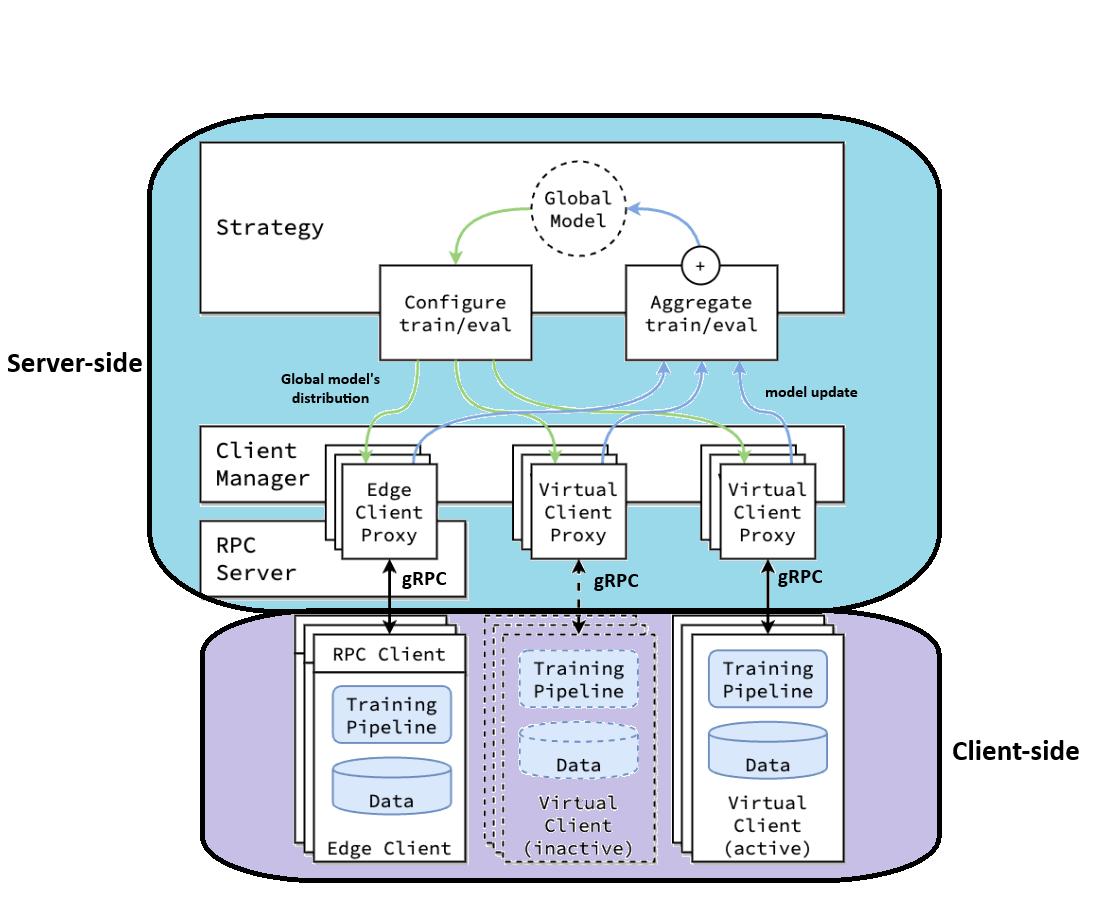
\includegraphics[width=.8\textwidth]{figures/tools/architecture_1.png}
    \caption{Flower architecture with a server, two edge clients and one virtual client.}
    \href{https://flower.ai/docs/framework/contributor-explanation-architecture.html#flower-architecture}{Source}
    \label{fig:flower_architecture}
\end{figure}
\noindent
Based on \cref{fig:flower_architecture},
Flower's architecture can be decomposed in three major parts: the server-side, the client-side, and the interprocess communication protocol.

The server-side contains the \emph{global model}, the \emph{strategy}, the \emph{client-manager} that orchestrates the \emph{client-proxies} and an \emph{RPC server}.
Strating from the \emph{global model}, it is computed by aggreagating the local updates and then redistributed to client following the FL process.
The management of the overall federated learning process, including configuring training/evaluation tasks and aggregating results from clients to update the global model
is assigned to the \emph{strategy}, that can be a pre-built implementation of a custom logic implemented by the user.
The \emph{client proxiestext}, represent an instance of the clients in the server side and  act as an intermediary between the RPC server and the edge clients, facilitating communication
and data exchange with gRPC call. The \emph{client-manager} assumes the responsibility of coordinating the interactions between the server and cients. Finally the \emph{RPC server}
handles remote procedure calls, enabling communication between the central server and distributed clients.

The client-side of the Flower framework consists of numerous clients, which can be either \emph{virtual} instances or \emph{actual edge devices}. Each client possesses a
\emph{local dataset} used for the local training process. In any given training round $r$, a client may be either \emph{active} or \emph{inactive}. Active clients, whether virtual or edge devices,
participate in the training process using their local training pipeline, which can be implemented on their preferred platform. Upon completing training, active clients
communicate their results through the \emph{RPC client interface} . Inactive clients remain dormant until they receive a gRPC call from the server, requesting their participation
in the subsequent round.

Finally the interprocess communication is conducted with the empolyement of the \emph{gRPC protocol}. In a brief summary, the protocol requires an RPC server on
the server-side and an RPC client on the client side. The RPC Server sends requests and receives responses from the RPC Client on the client-side.
Active clients use the gRPC protocol to send their local training results back to the server, ensuring efficient and reliable data transmission.
Inactive clients remain dormant until they receive a gRPC call from the server, prompting their participation in the next training round.
This mechanism supports seamless and scalable federated learning.

%%%%%%%%%%%%%%%%%%%%%%%%%%%%%%%%%%%%%%%%%%%%%%%%%%%%%%%%%%%%%%%%%%%%%%%%%%%%%%%%%%%%%%%%%%%%%%%%%%%%%%%%%%%%%%%%%%%%%%%%%%%%%%%%%%%%%%%%%%%%%%%%%%%%%%%%%%%%%%
% Network Simulator
\section{NS3: An Event-Driven Network Simulator}
\label{sec:ns3}
\href{https://www.nsnam.org/}{NS-3} is a discrete-event network simulator primarily used for research and educational purposes. What that means is that the simulator
models the operation of a network as a sequence of events occurring at specific points in time. Each event represents a distinct change in the state of the system,
such as the arrival of a packet, the completion of a transmission, or the movement of a node. The simulator processes these events in chronological order, updating
the state of the network accordingly. This approach allows for detailed and accurate simulation of network behavior over time.

Being open-source and highly extensible, NS-3 provides a realistic simulation environment for modeling and analyzing the performance of networking protocols and architectures.
It supports a wide range of communication topologies, both wired and wireless, with detailed implementations that manage various network layers to closely approximate
real-life setups. Notably, in wireless topologies, NS-3 can simulate node mobility, interference, and signal propagation.

Additionally, NS-3 offers traffic patterns, data flows, and traffic generators to experiment with different scenarios. This capability allows users to create detailed
and accurate network architectures, from which they can extract significant performance metrics such as latency, throughput, and jitter. These features make NS-3 a
powerful tool for investigating and simulating various networking scenarios, providing valuable insights into network performance and behavior.

NS-3 benefits from an active community of researchers and developers who continuously strive to enhance the accuracy of its models and the overall functionality
of the simulator. It offers comprehensive documentation, tutorials, and example scripts to assist users in getting started. The simulator is designed to be
user-friendly, featuring a modular architecture that facilitates easy integration and customization. Moreover, NS-3 supports interoperability with real-world
systems and other simulators, thereby enhancing its utility for diverse networking research and development projects. These attributes have established NS-3 as
a leading paradigm in the field, extensively used and taught in universities to foster research and education.

\section{Posix Sockets \&\ gRPC}
\subsection{Posix Sockets}
\href{https://www.wikiwand.com/en/Berkeley_sockets}{Posix Sockets}
are fundamental to network communication, providing a mechanism for two machines to exchange data over a network. Essentially, sockets offer a well-established API for
inter-process communication in internet and Unix Domain applications. They present the abstraction of a local endpoint in the communication path, represented as file descriptors.
Sockets use the TCP/IP protocol suite for communication and support both connection-oriented (using TCP) and connectionless communication setups (using UDP).
% and well-tested
The robust and reliable mechanisms of POSIX sockets make them a viable choice for federated learning (FL) inter-process communication. One major property of sockets,
making them suitable for FL setups, is their ability to handle both blocking and non-blocking communication enabling them to support synchronous and asynchronous FL.
In a blocking operation, the program halts until the entire message is sent or received, which can cause potential delays. Conversely, in a non-blocking operation, the
program sends or retrieves only the data that is immediately available, preventing it from stalling on slow connections and avoiding many deadlock situations.
% However, non-blocking operations do not guarantee that messages, especially large ones, will be sent or received in one piece. This trade-off allows for greater efficiency
% but requires careful handling of message integrity.

In our case, socket communication is restricted to operations within the NS-3 simulator, specifically handling the internal processes and simulations. This includes managing
the simulated network events and data exchanges. Once the simulation tasks are completed, sockets are used to communicate the results from NS-3 to the Flower framework.
This ensures that the network simulation outcomes are efficiently transferred for further processing in the federated learning workflow managed by Flower, enabling seamless
integration and coordination between network simulations and machine learning tasks.

\subsection{gRPC}
\href{https://grpc.io/}{gRPC}
is an open-source RPC (Remote Procedure Calls) framework developed by Google, designed for efficient, low-latency communication between distributed systems.
It allows a client to call methods on a server as if they were local, using Protocol Buffers (protobufs) for serializing structured data, ensuring fast and compact
communication. gRPC supports multiple programming languages and offers features such as authentication, load balancing, and bidirectional streaming, making it
ideal for microservices architectures where seamless and scalable service communication is essential. Its high performance and ease of integration make gRPC a popular
choice for modern distributed computing environments.

The process of RPC communication with gRPC begins by defining a service in a \emph{.proto} file using Protocol Buffers syntax, where service methods and message types are
specified. This definition is compiled using the protoc compiler to generate both client and server code. The server implements the service by providing the logic
for handling RPCs, processing requests, and sending responses. Meanwhile, the client creates a stub from the generated code, enabling it to invoke remote methods
on the server as if they were local functions.

It is important to clarify tha this context, "server" and "client" are used in a general sense for communication purposes, not specifically for federated learning
structures. The reason for this comment will be better demonstrated with the following example.

In our project the server orchestrates training and evaluation, maintaining client stubs within the client proxies. This setup allows the server
to remotely call the clients' fit and evaluate methods to initiate the learning process. Once the results are generated, they are returned to the client proxies and
subsequently to the server. Here, the client proxies, and indirectly the Flower server, function as the gRPC client, while the Flower clients act as the gRPC server.



